
\chapter{Intake and super/turbo charging}
\section{Torque curve}
	\wrapfig{7}{l}{3}{0.15}{ch7/1}{ch7/1}
	The maximum torque and power have this shape. To see why, let's define the \textbf{volumetric efficiency}: 
	
	\begin{equation}
	\sigma = \frac{m_{air,real}}{m_{air,theoretical}} = \frac{p \frac{V_{cyl}}{rT}}{p_{ref} \frac{V_{cyl}}{rT_{ref}}}
	\label{eq:7.1}
	\end{equation}
	
	the reference values are chosen as those at the intake. 
	
	\ \\
	
	\wrapfig{7}{r}{5}{0.15}{ch7/2}{ch7/2}
	This can be represented as A on the graph, but there is many losses: B charge heating because the lower the rpm the more time we heat the gas; C viscosity, D chock at high rpm, E back flow due to overlap, the rest is second order losses. We can see that the shape is very similar to the torque curve, the most we admit mass, the most we have torque. The length of the intake pipe plays also a role. The reason is that consider a cycle, when the valve is closing, the intake is disrupted and this creates a pressure wave in the pipe.
	\ \\
	
	\wrapfig{7}{l}{4}{0.15}{ch7/3}{ch7/3}
	 This will travel until the other side of the pipe and will be reflected. If the valve is open when the wave reach again the valve, there will be a pressure boost, increasing mass, increasing torque. This is called \textbf{engine acoustic}, the wave propagates at speed of air. The pipe design is used to modify the torque curve. This can be used in multicylinder engine but it is more complex since the wave can be used for another cylinder. And we can play with it: change of the length of the pipe (natural frequency), change between 3 cylinder acoustic and 6, allowing to modify the torque shape continuously. 
	 
\section{Valves}
	\wrapfig{3}{r}{4}{0.15}{ch7/4}{ch7/4}
	The valve is a nozzle that creates pressure losses, so it is designed carefully. Consider the radius $R$ and the lift $l$, the area can be approximated by a cylinder surface: 
	
	\wrapfig{4}{l}{3.5}{0.3}{ch7/5}{ch7/5}	
	\begin{equation}
	A_c = 2 \pi R l \qquad \Rightarrow A_e = C_D A_c
	\end{equation}
	
	where $A_e$ is the effective area taking into account the corrective factor for aerodynamic configurations $C_D$ (discharge coefficient). The maximum voluetric efficiency is obtained with maximum area, this is why we don't have straight valves in gasoline engine and the combustion chamber is in the cylinder head. The intake valve is the bigger one to make the intake easy, but has to be not too big because of the cooling issues. 
	\ \\
	
	\wrapfig{9}{r}{7}{0.3}{ch7/6}{ch7/6}	
	The working principle is exposed on the figure, we have \textbf{camshafts} turning with the engine that manage the opening/closing. Increasing the number of valves increases the cost since we need more camshaft. We could also use a single camshaft for both input and output valves but the force will be higher and will limit the lift size, thus the efficiency. But having 4 valves makes the torque higher than 2 valves, increasing the cost. 
	\ \\
	
	\wrapfig{8}{l}{5}{0.2}{ch7/7}{ch7/7}	
	The lift law is linked to the camshaft. Valve timing is driven by mechanical stress on camshaft and by pressure waves. There is an overlapping, generally not a problem, but we can play with it for example by trapping the gases in the cylinder after the exhaust (shift of intake on the right). This is called \textbf{Internal gas recalculation} (IGR) and it lower the efficiency. If we shift the intake to the left, the gases are flowing from inlet to outlet thus this is only used in direct injection to increase the performances, otherwise fuel to the exhaust. A way to use the acoustic waves is to shorter the compression stroke (Atkinson cycle better efficiency). 
	
\section{Control of the torque}
\subsection{Gasoline}
	\wrapfig{6}{l}{2.5}{0.2}{ch7/8}{ch7/8}	
	We can compute it as: 
	
	\begin{equation}
	P_{out} = \eta P_{fuel} = \eta \dot{m}_{fuel} LHV \propto \eta \dot{m}_{air} LHV \phi \quad \Rightarrow T_{out} \propto \eta \dot{m}_{air} LHV \phi
	\label{eq:7.3}
	\end{equation}
	
	so we see that we can play on the mass flow of air, this is done by cam profile or by intake pressure. Intake pressure is varying by means of the \textbf{throttle}. Impossible to change the equivalence ratio a lot because of the pollutants. 
	
	\minifig{ch7/9}{ch7/10}{0.2}{0.2}{0.2}{0.32}
	The problem with the throttle is that it increases significantly the pumping losses due to pressure losses. At the limit case of idle, we are still consuming because we counteract the pressure loss. Another way of controlling the torque is based on the lift size as shown on the second figure but this is more and more complex. 
	
\subsection{Diesel}
	First of all, there is less acoustic waves here because turbochargers kill it and the valve timing is limited by the piston motion. Indeed the compression ratio is much higher than in gasoline case, the piston head must be flat and thus the valve straight. The cylinder head - piston clearance is 0.7 mm, the valve should be closed when at TDC. It is thus very difficult to use waves to play on the shape of the torque, the area for the valve is limited, ... The volumetric efficiency of the diesel engine is limited to 0.7 without turbocharger (against 0.9 for gasoline). We will see that the shape of the torque curve is controlled with the \textbf{turbocharger}. \\
	
	\wrapfig{5}{l}{3}{0.3}{ch7/11}{ch7/11}	
	There is no camshafting or any fancy device on diesel since we have the turbo. For what concerns the number of valves, with 2 there is not a good swirl (aerodynamic) at every regime and lead to bad combustion. Valves are very important to generate turbulence via high speed air intake. In gasoline the main is \textbf{trumble} and for diesel, \textbf{swirl} for the mixing.   
	
\section{Turbocharger}
	\minifig{ch7/12}{ch7/13}{0.2}{0.2}{0.4}{0.35}
	
	One expects that the diesel engine will provide more torque than the gasoline because of the higher pressure ratio. But if we look to the equivalence ratio, due to soot limit $\lambda = 0.7$ for diesel and 1 for gasoline. 30\% of the air is not used. The diesel engine should thus provide less torque and power \eqref{eq:7.3}. \textbf{But this is not the case! Because we love turbochargers <3}. This consists in increasing the air mass flow in the same equation, by increasing the inlet pressure \eqref{eq:7.1}. This is done by transferring the exhaust expansion energy to the compression of the air. \\
	
	Compressing increases the temperature, we add an \textbf{intercooler} to reduce it (keep high $\sigma$). To avoid over regimes, the turbo is controlled (rpm between 100 000 - 300 000). 
	
\subsection{Description}
	\minifig{ch7/14}{ch7/15}{0.2}{0.2}{0.4}{0.25}
	Sleeve bearing or ball bearing, the first has more friction for low loads. The turbo is cooled by oil (all the oil flow pass from the turbo).  The main axle is linked to the turbine. Since the environment could be corrosive the material has to be chosen carefully (titanium for example) for the compressor represented on \autoref{ch7/15}. The turbo can only work on a limited range of rpm (we have to accelerate it). Small ones are easy to accelerate but compress less than a big one, which has more inertia and cannot rotate so fast. We define thus the \textbf{turbo lag}: 
	
	\begin{equation}
	T = I \frac{d\omega}{dt}
	\end{equation}
	
	where I increases and the other term decreases for big turbos. We can improve the turbo lag by for example adapting the incoming angle of the flow on the blades of the turbine or control the counter pressure coming from the exhaust. We could also use 
	
	\begin{itemize}
	\item[•] parallel sequential: use a small turbo for low mass flow and add one in parallel when higher
	\item[•] series sequential: replace the small one by a big one. \\
	\end{itemize}
	
	This is good for lag but it is difficult to control since there is valves everywhere. We could also try multiple turbos with each their own working range. If we go out of the region, the torque is hardly decreasing because of the stress on the engine. 
	
\paragraph{Industrial engines}
	They are turbocharged which gives them an advantage. They can compensate for hot and high conditions, which is not the case for gas turbine ! No fancy turbo, simple one, matched on the nominal regime. One waste gate and one intercooler, that’s all. Since mass flow is higher you can find axial turbine on BIG engines. The maximum torque of the diesel is more constant than the gasoline
	
\subsection{Gasoline engines}
	The main problem for the use of turbos on gasoline engines is the throttle. Indeed, the introduced pressure loss is too high. We can solve this problem by downsizing, which goal is to avoid at maximum the throttle. In fact, we use the turbo as a throttle. We have a smaller engine with smaller torque and instead of decreasing the manifold pressure with a throttle, we increase the manifold pressure in order to get higher torques. But the throttle is still present. \\
	
	In gasoline the mass flow ratio could go up to 80:1 while 6:1 in diesel, so the matching is more complex. Indeed we could combine variable valve lift, turbo, start stop, ...  
	
\paragraph{Some concerns}
	First of all, the use of turbo increases the knock sensitivity leading to downsizing even more, lower compression ratios and efficiency. Turbo charger has a protection for high rpm, thus we still need to use the throttle when the turbo is turning. \\
	
	Knock sensitivity can be reduced by reducing the compression ratio, changing the cycle (exhaust valve open during compression start). The turbo protection requires temperature maximum, the exhaust temperature minimal we can get from downsizing is still high. We can decrease it by adding more fuel! But this is lost fuel.  \\
	
	\textbf{Turbochargers only increase performance and not the overall engine efficiency.}
	
\section{Compressor}
	\wrapfig{5}{l}{6}{0.14}{ch7/16}{ch7/16}	
	This is another way of increasing the input air, before the turbo. It consists in compressing the air but linked to the crankshaft. For aero engine in the 1930s for example there were centrifugal compressors. 
	
	\ \\\\
	
\paragraph{The roots compressor}
	\begin{wrapfigure}[7]{r}{4cm}
	\vspace{-20mm}
	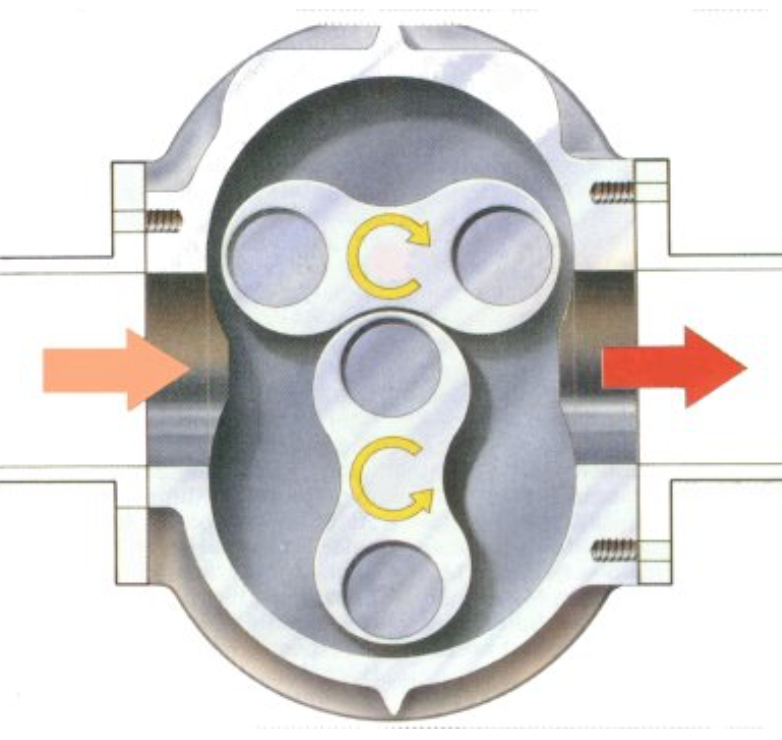
\includegraphics[scale=0.3]{ch7/17}
	\captionof{figure}{}	
	\end{wrapfigure}
	Rotation is given by the crankshaft. Since there is no volume change, pressure ratio is limited. Isentropic efficiency is very low and there are leaks, reducing further the efficiency. There is an increase in kinetic energy due to the lobes rotation, then a sudden transition from kinetic to pressure energy which is bad for efficiency, on a turbo the volute is responsible for energy conversion. Always coupled with an intercooler. \\
	
	Further \textbf{helicoidal} roots have been developed, making the transition between kinetic and pressure energy smoother. Its efficiency is as high as the turbo compressor. This is sometimes used in engines nowadays, since there is no change in efficiency but the cost is lower. Since it is linked to the crankshaft rotation, the use of a throttle is tricky. But it needs recirculation, the compression ratio is low and thus cannot be used to boost on diesel. \textbf{The main advantage is the very very low response time, allowing to boost the torque at low rpm}. \\
	
	A turbocompressor (CVT) can also be used, it is a turbo linked to the crankshaft, giving low response time, but rotation speed much lower. The gain in response time can also be performed by electric drive compressor.  
	
	
	\minifig{ch7/18}{ch7/19}{0.15}{0.15}{0.35}{0.3}
	The expansion of exhaust gases reduces the temperature and could be not good for the catalyst effect. For a 2 strokes engine the only device to use is the \textbf{supercharger} (turbocharger uses the exhaust gas). Indeed, since the exhaust is performed by means of the piston motion, it is bad to put counter pressure at the output. 
	
	\minifig{ch7/20}{ch7/21}{0.2}{0.18}{0.49}{0.49}

	
